\documentclass[12pt]{article}
\usepackage{zed-csp}
\usepackage[top=1.5cm, bottom=1.5cm, left=2cm, right=2cm]{geometry}
\usepackage{graphicx}
\begin{document}

\begin{Huge}
\begin{center}
\begin{normalsize}
\textbf{MAKERERE 
\includegraphics[scale=0.5]{logo} UNIVERSITY }\\


\textbf{FACULTY OF COMPUTING AND INFORMATICS TECHNOLOGY} \\
\textbf{SCHOOL OF COMPUTING AND INFORMATICS TECHNOLOGY} \\
\textbf{DEPARTMENT OF COMPUTER SCIENCE} \\
\textbf{BACHELOR OF SCIENCE IN COMPUTER SCIENCE} \\
\textbf{YEAR 2} \\
\textbf{BIT 2207 RESEARCH METHODOLOGY} \\
\textbf{Course Work: Proposal Assignment }\\
\end{normalsize}
\end{center}
\end{Huge}

\begin{center}
\begin{tabular}{|l|l|l|c|}
\hline NAME  & REG NO & STD NO \\\hline

ABILA Raphael& 16/U/2673/PS & 216006923 \\\hline
MWAITA Joshua& 16/U/7890/PS & 216018350 \\\hline
NAKAFEERO Peninah&16/U/8463/PS & 216009254 \\\hline
OJIAMBO ABEX     & 16/U/10829/PS & 216013324 \\\hline
\end{tabular}
\paragraph{•}
Lecturer: ERNEST MWEBAZE \\
\paragraph{•}
18th April 2018

\end{center}

\vspace{6cm}

\title{}\textbf{\textbf{AUTOMATED WEB APPLICATION SYSTEM TO IMPROVE ON PATIENTS’ APPOINTMENT WITH DOCTORS TO REDUCE DEATHRATES OF CANCER PATIENTS IN UGANDA.}} 

\newpage




\section{Introduction}
\subsection{Background}

\paragraph{}Cancer has become an epidemic that is on a high rise in the recent years and there are not so many hospitals that have proper facilities well equipped to have this disease treated properly and mortality rates are rising as the victims are taken to their early graves as due to a lack of proper treatment since well-defined information details about these Cancer oncologists specialised in treating Cancer in Uganda.

Cancer can be detected if one goes for image scans like X-rays, CT, MRIs, radionuclide bone and positron emission tomography (pet) scans as well as biopsy which can clearly be used to clearly identify the presence of cancer cells.

Discovering that one has Cancer is tiresome and frustrating more so when finding the medical specialists and getting treatment for the Cancer for example one has to move from their home areas to the Uganda Cancer Institute at Mulago national referral hospital to acquire treatment which is very costly and cumbersome to patients all due to the limited ways of acquiring all this information about the specialists who have established themselves with good years of experience and health institutes for the treatment of Cancer is limited in Uganda mostly known to be stationed in Kampala.

The automated web application system will help narrow this inadequacy of information about these oncologists in Kampala and Uganda defining their details of location, office contacts, hospital base of practice.

\subsection{Problem Statement}
\paragraph{•}Limited access to Cancer medical specialists’ information by the general public. This is due to inadequate access and availability of Cancer specialists information in the country making the existing system very hard to work with and very costly in terms of having access to information about cancer oncologists, well trained to treat cancer in registered hospitals  ,patients are forced to move up to the hospitals for information inquiry thus the need for the development of a new system of accessing this information at their comfort.

\subsection{Main Objective}
\paragraph{•}To develop an automated web application system in an information deprived environment to provide information to the public about these oncologists to their conveniences.


\subsection{Specific Objectives}
\paragraph{•}The Specific Objectives of the study are as follows:
\\i.	To investigate the challenges of the current system and collect user requirements for the development of the automated web application system.
\\ii.	To analyse and determine the user requirements for the automated web application system.
\\iii.	To design and implement the automated web application system to meet the above the system requirements for the specified disease medical specialists in Uganda.  
\\iv.	To test and validate the implemented automated web application system with the proposed users.

\subsection{Scope}
\paragraph{•}The project was meant to produce a web application to //help users or patients to find Cancer medical specialist. Some hospitals and institutions like Mulago and Uganda Cancer Institute were visited within Kampala in order to find out better information of their views on the proposed project.

\subsection{Significance}
\paragraph{•}The research will provide these benefits;
\\{•}i. It will also increase efficient patient treatment progress closely across their locale and provision of professional guidance to the patients.
\\{•}ii. It will provide easy and quick information access to anyone in need of the Cancer medical specialist details.
\\{•}iii. It will also provide patients an easier means to locate their doctors with the detailed working schedules and appointment hours and a chat-room platform with their medical specialists in relation to their conditions.
\\{•}iv. To increase wide spread public awareness about cancer and productive information to control and prevent late cancer detections among Ugandans.
\\{•}v. It will also help patients access these medical specialists easily in accordance to their working hours with the appointment system installed in the web system increasing doctor access to patients.


\section{Literature Review}
\paragraph{•} Many studies have been made on cancer although the literature covers many theories and scientific facts about what cancer is all about, this review will focus on the patient and their need and how Information Technology (IT) can bridge the gap of psychological, emotional, medical and possibly physical needs that affect the daily lives of Cancer patients and how best they can get help from Cancer specialists and other medical stake holders like counsellors. 

The Psychosocial Needs of Cancer Patients elaborates that cancers historically have not been thought of as chronic diseases, they increasingly meet the definition of chronic diseases: “They are permanent, leave residual disability, are caused by nonreversible pathological alteration, require special training of the patient for rehabilitation, or may be expected to require a long period of supervision, observation, or care”\cite{Timmreck} even after completing treatment.

Cancer has Induced Physical Stress such as health impairment, Disability, Fatigue and Pain.Fatigue is the most frequently reported symptom of cancer and is identified as causing the greatest interference with daily activities of patients, although estimates of rates of fatigue among individuals with cancer vary greatly (ranging, for example, from 4 percent in breast cancer patients prior to the start of chemotherapy to 91 percent in breast cancer patients after surgery and chemotherapy and before bone marrow transplantation). Fatigue is theorized to arise from a complex combination of poorly understood physical and psychological effects of illness that may be different in each patient\cite{Carr}. An estimated one-third to one-half of patients undergoing active treatment for cancer experience pain resulting from the illness. Its treatment or co-occurring illnesses. This pain often is not fully eliminated despite the administration of analgesics and other therapies, in part because it is often undertreated. Moreover, pain may continue to be a problem even when there is no longer any sign of cancer. AHRQ’s 2002 evidence review documented the contribution of cancer-related pain to fatigue, impaired function, and a range of other psychosocial dimensions of health\cite{Carr}.

\subsection{Limitations in Activities of Daily Living.}

\paragraph{•}The physical impairments and disabilities, as well as fatigue and pain, experienced by patients with cancer often lead to an inability to perform the routine activities of daily living that most people take for granted. Activities of daily living are defined as those age-appropriate physical and cognitive activities that individuals generally perform for themselves as part of their daily self-care such as bathing, using the toilet, dressing, preparing meals, and feeding oneself. NHIS data for 1998 to 2000 show that cancer survivors without any other chronic illnesses were more than twice as likely as individuals without a history of cancer or other chronic illness to report limitations in their ability to perform activities of daily living and significantly more likely to have other functional limitations \cite{Hewitt}. 

\subsection{Web applications} 
\paragraph{•}The revolutionary break through that enabled computer designers to miniaturise circuit boards gave birth to a new breed of computers that were much smaller, portable and convenient to use thus the rise of mobile computers. These mobile computers needed applications to facilitate their usability. In the beginning companies used their own developers to make applications but as the demand outstripped the supply of the applications the application development process had to be made open source which has given rise to the rich and vast web application markets. However this could not be possible without the operating systems that the mobile computers run on.

\subsubsection{Existing Systems vs the Web Application}
\paragraph{•}Manual Method: This is the most used system in Uganda today. It involves physically travelling to the hospitals and inquiring on when and how one can access specific medical experts. 

Cancer.Net: This is an online web system (plus a web application) that enables users around the world to access detailed information about all types of cancer the world. With nearly 40,000 members who are leaders in advancing cancer care, the American Society of Clinical Oncology (ASCO) is the voice of the world’s cancer physicians.

The Web application : Our web application for locating Cancer specialists puts together the benefits of the top two systems and adds to that. First, its online 24/7, thus users can contact specialists at their own time of convenience without having to wait in long queues for ages. 


\paragraph{•}\textbf{CONCLUSION}
The Web App is a high end application that has practical application in third world countries to suit the needs of Cancer patients with the most convenience.

\section{Methodology}
\paragraph{•}This section describes the step by step process that will be followed to achieve the project specific objectives. This study will involve both qualitative and quantitative methods.
This is because the research requires people’s views and opinions, and analysis of documents.

\subsection{Data Collection}
\paragraph{•}In order to identify system requirements, data was collected and analysed. Data collection and analysis techniques that were used include.

\subsubsection{Interviews} 
\paragraph{•}Four (4) Cancer patients were interviewed using face to face interactions. This enabled getting of real information on the problems they face in finding Cancer specialists, procedures they took and how long it took to report and locate the specialists.
\\The interview method was chosen since most parents were more comfortable expressing their experience verbally as compared to filling in questionnaires. 

\subsubsection{Observation}

\paragraph{•}There is a lot of bureaucracy in finding medical specialists where the patients are required to spend hours in line, moving from office to office, making calls and at times bribing the people in charge in order to get through to the specialists. 

\subsection{System Analysis and design}  
\paragraph{•}System analysis was done using level 1 Data flow diagrams to show overview of the Web Application system, identifies major processes and data flows between them and identifies data stores that are used by the system.
 
\begin{center}
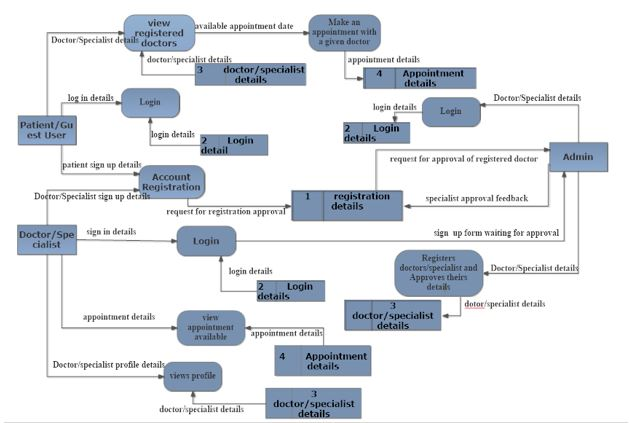
\includegraphics[scale=0.5]{dfd}
\end{center}

 System design includes the process and data modelling of the Web application system and below is the architecture of the system.
 
\begin{center}
\includegraphics[scale=0.5]{architecture}
\end{center}


\subsection{Implementation}
\paragraph{•}This stage is where visions, plans become reality. This is the logical conclusion, after evaluating, deciding, visioning, planning, applying for the proposed project. This process involves having an action plan in place, achieving tangible change and improvements from one stage to another, ensuring that any unforeseen conflicts that might rise are neutralized before continuing to the next phase or stage.
\subsubsection{Tools to be used}

\paragraph{•} HTML 5:  A revision of the Hypertext Markup Language (HTML), the standard programming language for describing the contents and appearance of Web pages. 

PHP:  The application database was linked using PHP scripting language. PHP was used to develop scripts that connected and pulled data from the database and display it in the system. 

MySQL: This is a relational database management system that is open source and free, runs on all platforms available and its able to handle large data manipulations.

JAVASCRIPT: JavaScript is a client- side scripting language used because of its ability to handle form processing burden and it promotes dynamism.

CSS: This was used because of its dynamism to separate content from the design in order to make the design work simpler for example the colour, font, text, and many more.

\subsubsection{System Testing} 
\paragraph{•}Testing is the process of executing the application programs with the intent of finding errors and observing if it is behaving as expected. Testing of the design will be first done by the developers and then take it to the users for testing. The following testing methods will be used;

\paragraph{•}i.	 Unit Testing: This is the process of testing the individual units of source code to determine if they are fit for use. A unit is the smallest testable part of an application.

ii.	System Testing : This is a complete replication of the running system for purposes of testing out the adequacy of the system. 

iii.	Compatibility testing: This was done to ensure that the system is compatible with the windows operating system and protocols under which the data is to be transmitted. 

\subsection{Results or system functionalities}
\paragraph{•}The following screenshots are to explain the different user interfaces available in the proposed system which include: 

\paragraph{•}Patients / Users Home Page: Displays a welcome message created by the administrator.

\paragraph{•}user login: User must be logged in to complete the appointment booking

\paragraph{•}appointment module: Users are able to make appointments when they access this page.


\begin{center}

\includegraphics[scale=0.6]{home}
\end{center}

\begin{center}
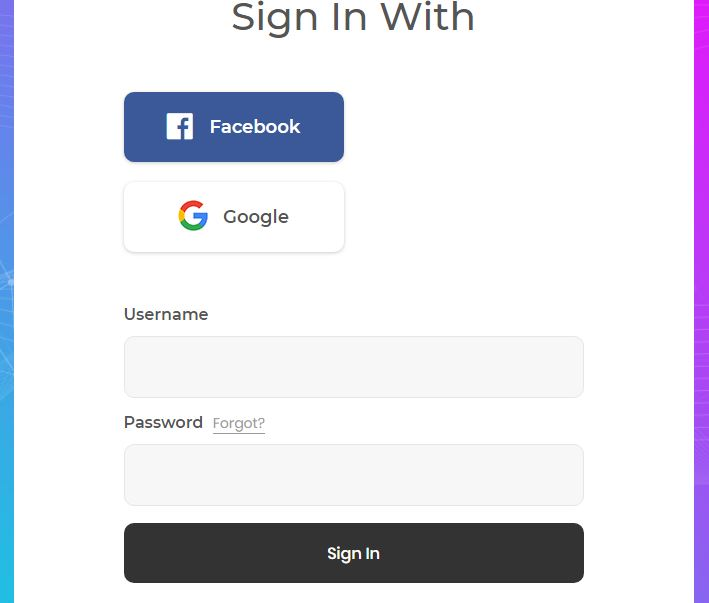
\includegraphics[scale=0.6]{loggin}
\end{center}

\begin{center}
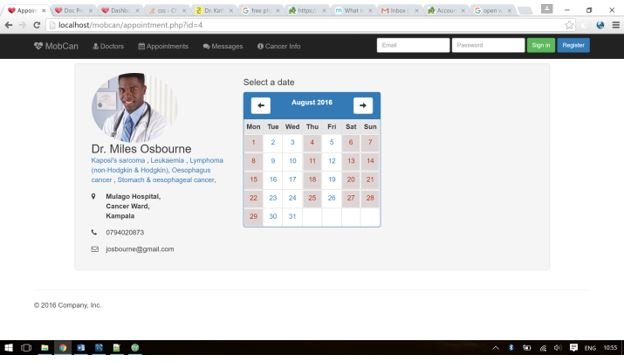
\includegraphics[scale=0.8]{appointment}
\end{center}


\begin{thebibliography}{9}

\bibitem{Timmreck} Prof. Timmreck. \textit{Demographic and Clinical Profile of Cancer Patients },Internet:https://awlworld.com/demographic-and-clinical-profile-of-cancer-patients-and-their-psychosocial-needs, August 26, 2017[April 18, 2018].


\bibitem{Carr} 
Carr-Schmid A, Pfund C, Craig EA, Kinzy TG. \textit{SGD},Internet:https://www.yeastgenome.org/reference/S000069709, August 26, 2013[April 18, 2018].

\bibitem{Hewitt}J Pers Soc Psychol. \textit{NCBI},Internet:https://www.ncbi.nlm.nih.gov/pubmed/12793591, June 6, 2003[April 18, 2018].



\end{thebibliography}


\paragraph{•}\textbf{APPENDIX}
\\i. Projected Cost For Development

\begin{center}
\begin{tabular}{|l|l|l|c|}
\hline NUMBER  & ACTIVITY & COST(Shs) \\\hline

1 & Gathering information & 150,000 \\\hline
2 & Design a framework & 100,000\\\hline
3 &Implementation & 200,000 \\\hline
4 & Miscellaneous & 200,000\\\hline
  & TOTAL & 650,000\\\hline
\end{tabular}
\end{center}

 ii. Questionaires

\paragraph{•}1. How long have you noticed the bone pain?
\\Why: to establish if acute or chronic.
2. Is the bone pain localized or generalized?
3. Is there a history of trauma or injury?
\\Why: may suggest fracture. If the injury was minimal may suggest osteoporosis or pathological fracture due to bone tumour or bone metastases.
4. Is the bone pain present day at night?
\\Why: may suggest more serious cause such as bone tumour, bone metastases, leukaemia, Paget's.





\end{document}